% -*- program: xelatex -*-
\documentclass[11pt, compress]{beamer}

\usepackage{fontspec}
  
\setsansfont{PT Sans}
 \setmonofont{PT Mono}

\usepackage{beamerthemesplit}
\usefonttheme[onlymath]{serif}
%\DeclareFontEncoding{T1}
\fontencoding{T1}

%\usepackage[T2A]{fontenc} 
\usepackage[utf8x]{inputenc}
\usepackage[russian]{babel}
\usepackage{listings}

\usepackage{amsmath,amssymb,amsthm}
\hypersetup{unicode=true}
\usepackage{graphics,graphicx}
\usepackage{verbatim}
\usepackage{fancyvrb}
\usepackage{booktabs} 
%\usepackage{media9}
\usepackage[super]{natbib}
\usepackage{color}
\definecolor{mygreen}{RGB}{28,172,0} % color values Red, Green, Blue
\definecolor{mylilas}{RGB}{170,55,241}
\definecolor{codecolor}{RGB}{0,120,0}
\definecolor{light-gray}{gray}{0.95}
\definecolor{light-green}{rgb}{0.93, 1, 0.8}
\definecolor{light-yellow}{rgb}{1,1,0.85}
\definecolor{dark-blue}{rgb}{0,0,0.6}
\definecolor{dark-red}{rgb}{0.7,0,0.0}
\definecolor{dark-green}{RGB}{10,150,0}

\newcommand{\matcode}[1]{ \textcolor{codecolor}{\texttt{#1}}}


\usepackage{pifont}% http://ctan.org/pkg/pifont
\newcommand{\cmark}{\textcolor{green}{\ding{51}}}
\newcommand{\xmark}{\textcolor{red}{\ding{55}}}

\setbeamercolor{frametitle}{fg=dark-red,bg=gray!10}
\setbeamerfont{title}{series=\bfseries,parent=structure}
\setbeamerfont{frametitle}{series=\bfseries,parent=structure}

\setbeamertemplate{blocks}[rounded][shadow=false]
\setbeamertemplate{navigation symbols}{}

\newcommand{\code}[1]{\textcolor{dark-green}{\texttt{#1}}}
\newcommand{\cleartitlepage}[1]{\begin{frame}[plain]\begin{center}\textsc{#1}\end{center}\end{frame}}
\renewcommand{\emph}[1]{\textcolor{dark-blue}{#1}}
\newcommand{\emphb}[1]{\textcolor{dark-blue}{\textbf{#1}}}
\newcommand{\lstcomment}[1]{\textcolor{dark-green}{\texttt{#1}}}

\usepackage{dirtree}

\usetheme{CambridgeUS}
\usecolortheme{lily}

\lstset{basicstyle=\ttfamily,
    language=matlab,    
    keepspaces=true,
    extendedchars=\true,
    basicstyle={\small},
    breaklines=true,
    morekeywords={matlab2tikz},
    keywordstyle=\color{blue},
    morekeywords=[2]{1}, keywordstyle=[2]{\color{blue}},
    identifierstyle={ \bf \color{black} },
    stringstyle=\color{mylilas},
    commentstyle=\color{mygreen},%
    showstringspaces=false,
    numbers=left,%
    numberstyle={\scriptsize \color{gray}},
    numbersep=7pt, 
    emph=[1]{case,switch,otherwise,nonlocal,as,yield, with},emphstyle=[1]\color{blue}, 
    frame=single,    
    rulecolor=\color{red},    
    backgroundcolor=\color{light-gray},
    xleftmargin=0.3cm,
    frame=l,framesep=4pt,framerule=0.5pt,
    escapechar=|
    %lineskip=-1.0pt,
    %emph=[2]{word1,word2}, emphstyle=[2]{style},    
}

\usepackage{tikz}
\usetikzlibrary{calc,patterns,decorations.pathmorphing,decorations.markings,positioning}
\tikzset{cbutton/.style={rectangle,minimum width=10mm,thick,draw=red!50!black!50,
top color=white,bottom color=red!50!black!30}}
\tikzset{mbutton/.style={rectangle,minimum width=10mm,thick,draw=black!20,
top color=white,bottom color=black!30}}

\usetikzlibrary{arrows,shapes}
\tikzstyle{every picture}+=[remember picture]


\makeatother
\setbeamertemplate{footline}
{
  \leavevmode%
  \hbox{%  
  \begin{beamercolorbox}[wd=.3\paperwidth,ht=2.25ex,dp=1ex,center]{author in head/foot}%
    \usebeamerfont{author in head/foot}\insertshortauthor
  \end{beamercolorbox}%  
  \begin{beamercolorbox}[wd=.6\paperwidth,ht=2.25ex,dp=1ex,center]{title in head/foot}%
    \usebeamerfont{title in head/foot}\insertshorttitle
  \end{beamercolorbox}%
  \begin{beamercolorbox}[wd=.1\paperwidth,ht=2.25ex,dp=1ex,center]{date in head/foot}%
    \insertframenumber{} / \inserttotalframenumber\hspace*{1ex}
  \end{beamercolorbox}}%
  \vskip0pt%
}

\setbeamertemplate{headline}{}
%\setbeamertemplate{footline}{}
 
\AtBeginSection[]{
  \begin{frame}[plain]
  %\vfill  
  \begin{tikzpicture}
  \useasboundingbox (0,0) rectangle(\the\paperwidth,\the\paperheight);  
  \fill[color=dark-red]   (-1cm, 3.9cm) rectangle(\the\paperwidth, 5.9cm);
  %\usebeamerfont{title}\insertsectionhead\par%
  %\node[text width=\the\paperwidth,align=center] at (current page.center) {\color{ExecusharesWhite}\Large\textbf{\insertsectionhead}};  
  \node[text width=\the\paperwidth,align=center] at (6cm,4.9cm) {\color{white}\Large\textbf{\insertsectionhead}};  
  \end{tikzpicture}
  \end{frame}
}



% ============================================================================

\usepackage{tikz}
\usetikzlibrary{positioning} 
\tikzset{cbutton/.style={rectangle,minimum width=10mm,thick,draw=red!50!black!50,
top color=white,bottom color=red!50!black!30}}
\tikzset{mbutton/.style={rectangle,minimum width=10mm,thick,draw=black!20,
top color=white,bottom color=black!30}}


\tikzstyle{block} = [rectangle, draw, fill=yellow!20, text width=5em, text centered, rounded corners, minimum height=5em]
\tikzstyle{subblock} = [rectangle, draw, fill=white, text width=2em, text centered, minimum height=1em]
\tikzstyle{module} = [rectangle, draw, fill=none, text width=5em, text centered, rounded corners, minimum height=5em]
\tikzstyle{line} = [draw, ->]




\title{Интегрирование дифференциальных уравнений}
\subtitle{Основы MATLAB}
\author[Кафедра теоретической механики]{Юдинцев В. В.}
\small
\institute[СГАУ]
{
Кафедра теоретической механики
}
 
\begin{document}

{
\usebackgroundtemplate{
\includegraphics[width=\paperwidth,height=\paperheight]{back.png}}
\begin{frame}[plain]
\maketitle
\end{frame}
}


\frame{
\frametitle{Содержание}
\tableofcontents
}

%
%
%
\section{Интегрирование ОДУ}
%
%
%
\begin{frame}{Дифференциальные уравнения}
$$
\left\{
\begin{aligned}
& \frac{d q_1}{dt} = f_1(t,q_1,q_2,\ldots,q_n),  \\
& \frac{d q_2}{dt} = f_2(t,q_1,q_2,\ldots,q_n),  \\
& \ldots \\
& \frac{d q_n}{dt} = f_n(t,q_1,q_2,\ldots,q_n).  
\end{aligned}
\right. 
\quad \Rightarrow \quad
\frac{d \boldsymbol q}{dt} = \boldsymbol f(t,\boldsymbol q)
$$
где 
\begin{itemize}
  \item $\boldsymbol q = (q_1,q_2,\ldots,q_n)^T$ -- вектор состояния;
  \item $\boldsymbol f(t,\boldsymbol q) = (f_1,f_2,\ldots,f_n)^T$ -- вектор-функция правых частей.
\end{itemize}
\end{frame}

\begin{frame}{Алгоритм}
\begin{itemize}
  \item Приведение уравнений к системе дифференциальных уравнений первого порядка.
  \item Разработка файл-функции правой части $\boldsymbol f(t,\boldsymbol q)$.
  \item Разработка файл-скрипта запуска процесса интегрирвования ДУ.
\end{itemize}
\end{frame}

\section{Задача баллистики}

\begin{frame}{Пример: задача баллистики}
  \begin{figure}[htbp]
    \centering
    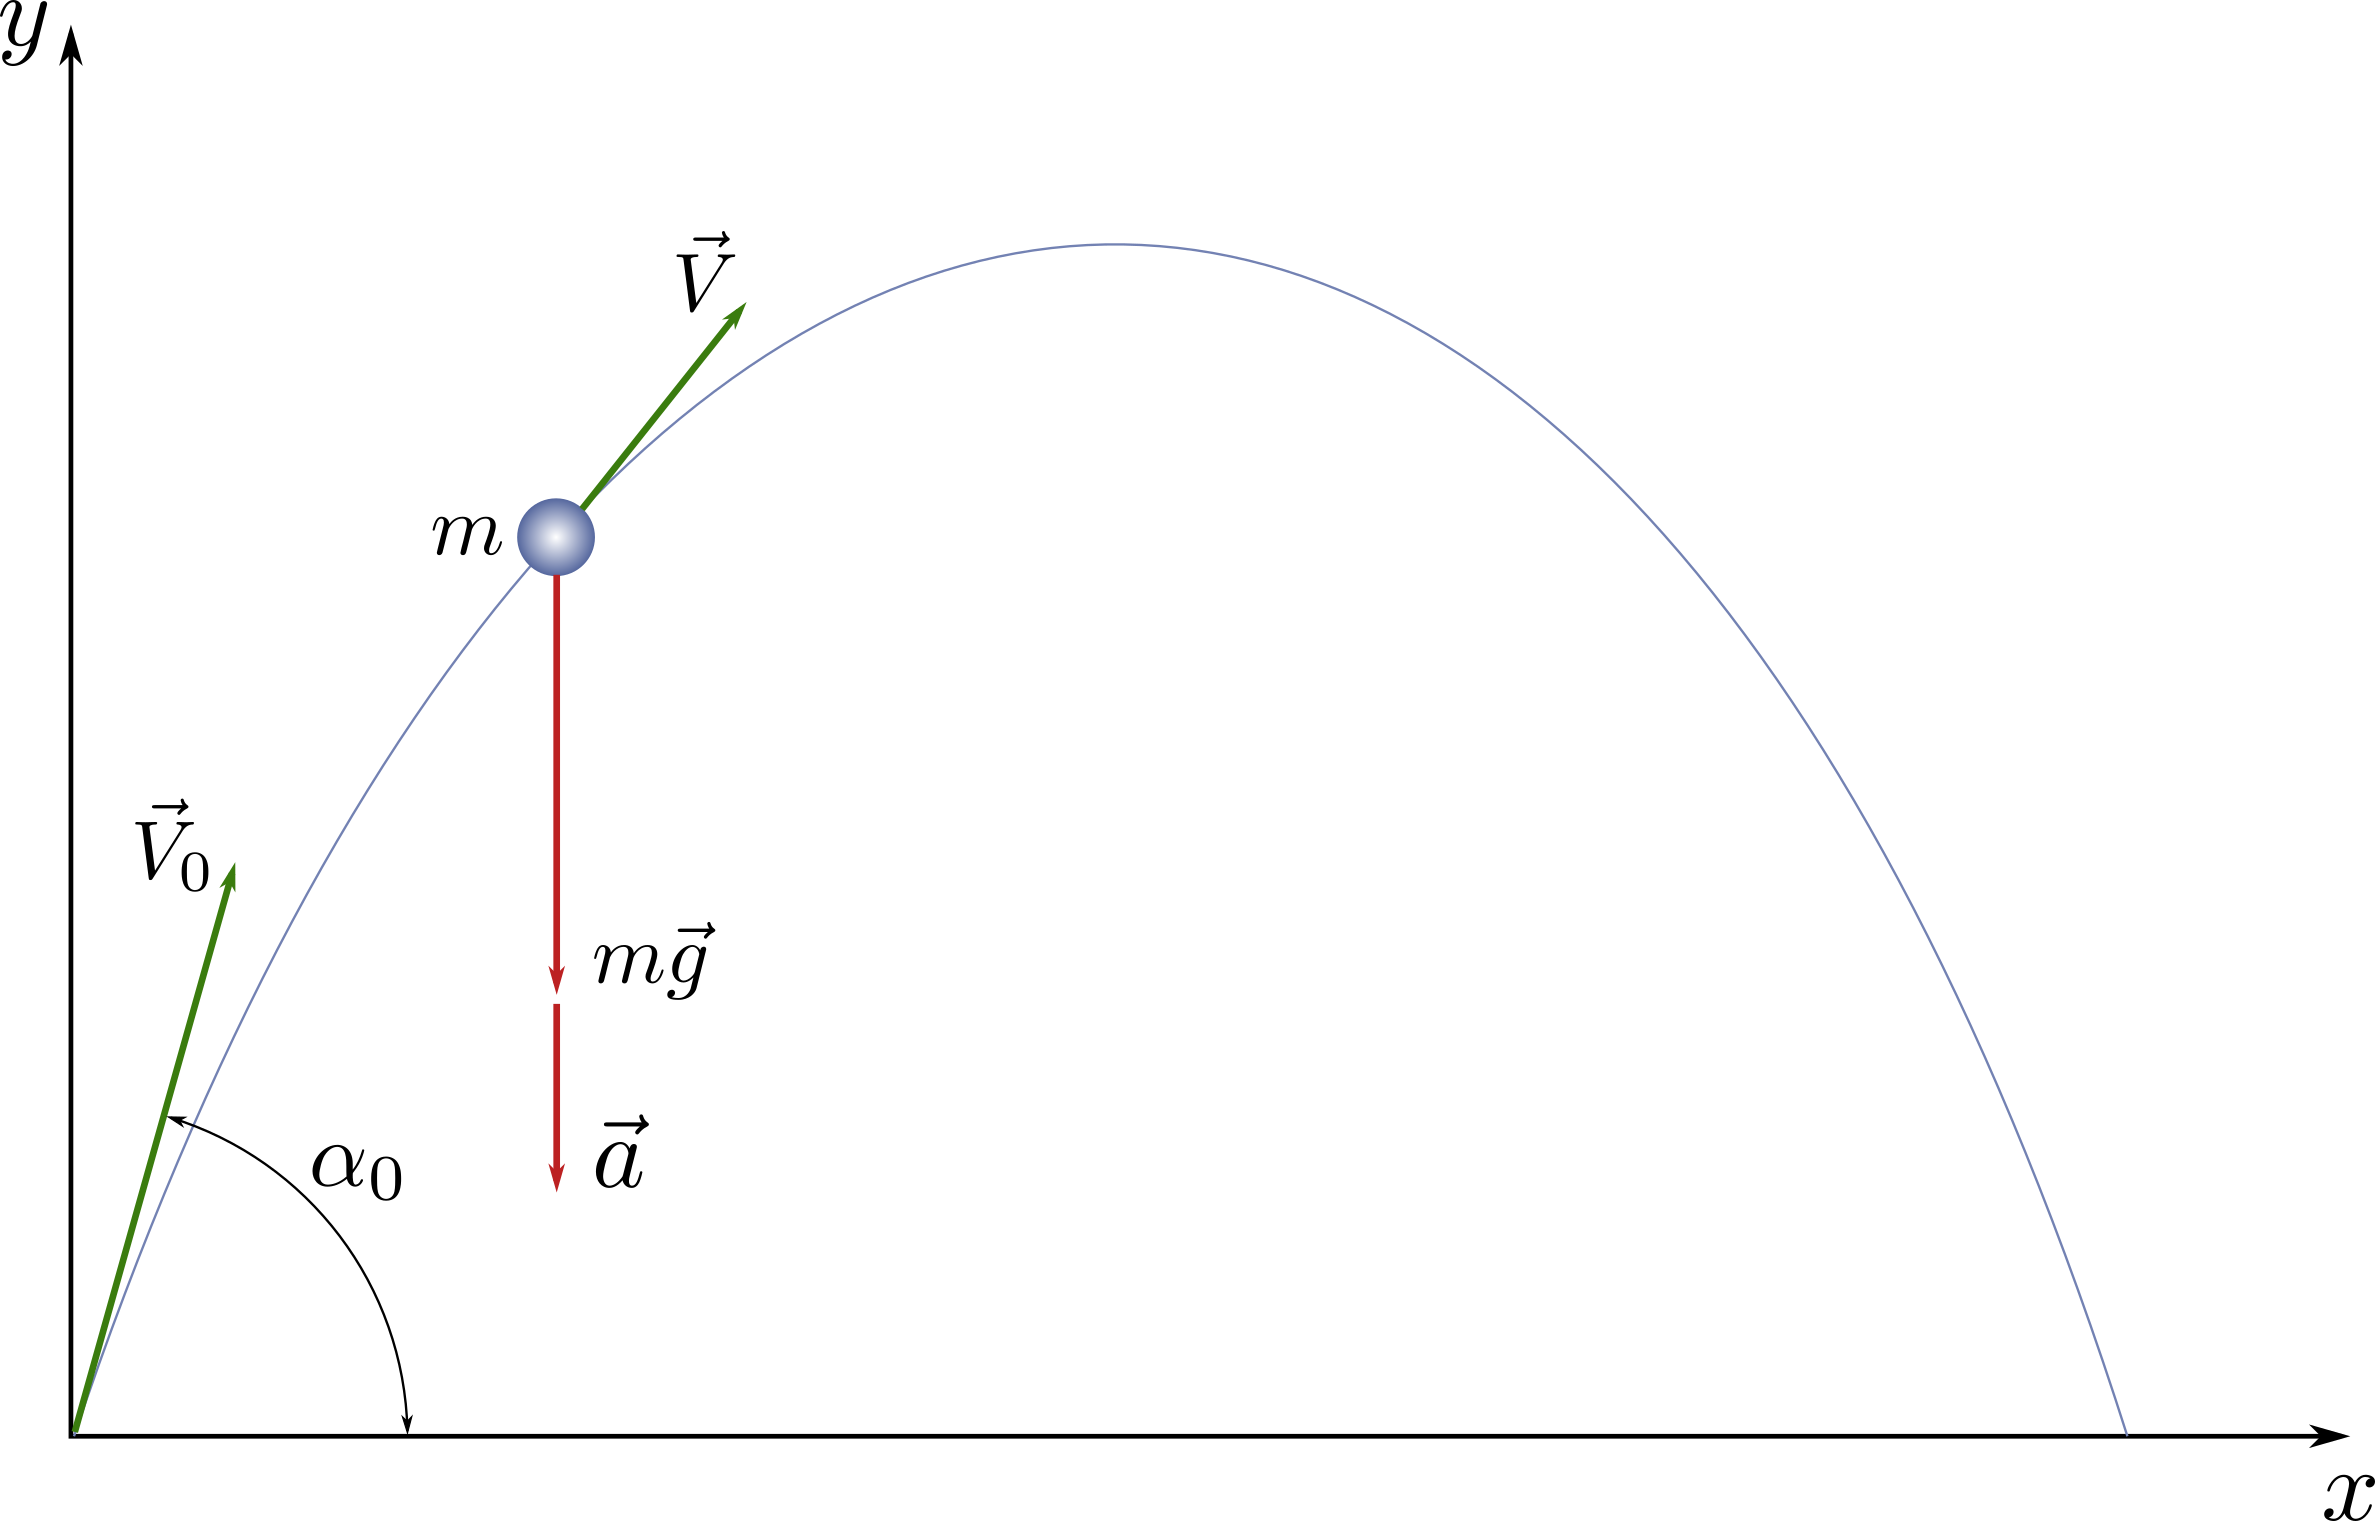
\includegraphics[width=1\textwidth]{Fall1.png}
  \end{figure}
\end{frame}

\begin{frame}{Уравнения движения}
\begin{columns}
\column{0.4\linewidth}
  \begin{figure}[htbp]
    \centering
    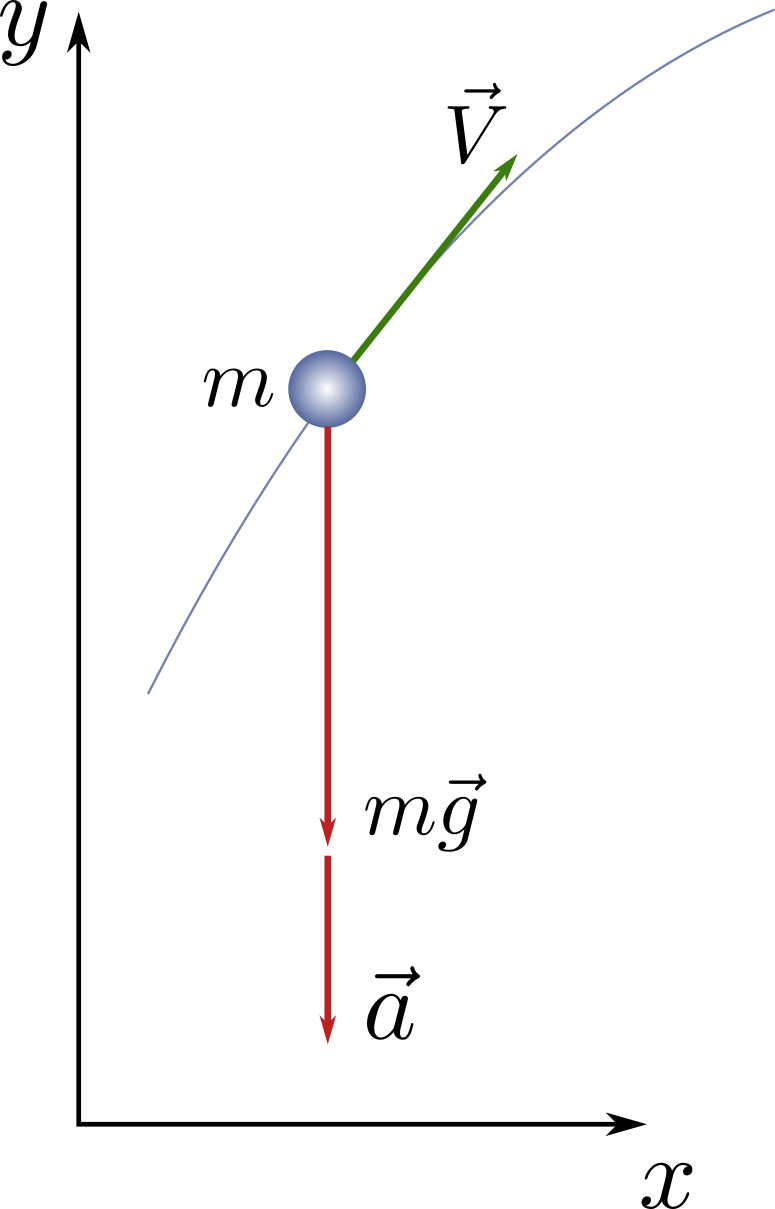
\includegraphics[width=1\textwidth]{Fall2.png}
  \end{figure}
\column{0.6\linewidth}
Векторное уравнение
$$
  m \vec a = \vec F_g = m \vec g.
$$  
Проекции векторного уравнения на оси координат:
$$
\begin{aligned}
  & m a_x = m \frac{d^2x}{dt^2} = 0, \\
  & m a_y = m \frac{d^2y}{dt^2} = - m g.
\end{aligned}
$$  
\end{columns}
\end{frame}



\frame
{
\frametitle{Дифференциальные уравнения движения}
Приведение к системе дифференциальных уравнений первого порядка.
$$
\left\{
\begin{aligned}
& m \frac{d^{\,2} x}{dt^2} = 0,  \\
& m \frac{d^{\,2} y}{dt^2} = - m g.
\end{aligned}
\right. 
\quad \Rightarrow \quad
   \left\{
   \begin{aligned}
   & \frac{d\alert{x}}{dt} = V_x,  \\   
   & \frac{d\alert{V_x}}{dt} = 0, \\
   & \frac{d\alert{y}}{dt} = V_y,  \\
   & \frac{d\alert{V_y}}{dt} = - g.
   \end{aligned}
   \right.
   \quad \Rightarrow \quad
   \frac{d \boldsymbol q}{dt} = \boldsymbol f(\boldsymbol q, t)
$$
где
$$
  \boldsymbol q=(\alert{x},\alert{V_x},\alert{y},\alert{V_y})^T, \quad \boldsymbol f(\boldsymbol q, t) = (V_x,0,V_y,-g)^T
$$
}


\frame[containsverbatim]
{
\frametitle{ODE файл -- файл-функция правых частей}
Файл в котором вычисляется правая часть дифференциального уравнения или системы уравнений:
$$
  \mathbf q \Rightarrow \boxed{ \dot{\mathbf q} = \mathbf f(\mathbf q,t) }  \Rightarrow  \dot {\mathbf q}
$$
где $\mathbf q$ -- вектор зависимых переменных, $t$ -- время.

Файл-функция \matcode{dqdt.m}
\begin{lstlisting}
function dq = dqdt(t,q)
  g = 9.81;
  m = 1.00;
  x=q(1); Vx=q(2); y=q(3); Vy=q(4);
  dq = [Vx, 0, Vy, -g];
\end{lstlisting}
}

\frame[containsverbatim]
{
\frametitle{Интегрирование}
Файл-скрипт основной программы (main.m)
\begin{columns}
\column{0.25\linewidth}
  \begin{figure}[htbp]
    \centering
    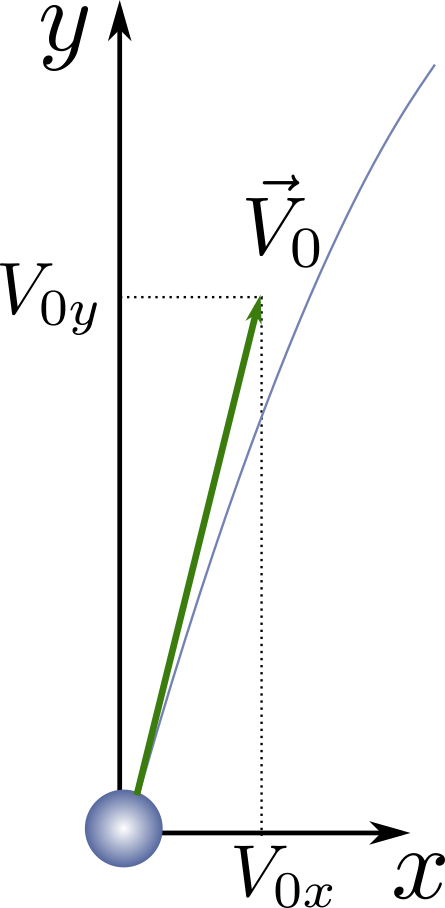
\includegraphics[width=1\textwidth]{Fall3.png}
  \end{figure}
\column{0.75\linewidth}
\begin{lstlisting}
% |\lstcomment{Начальные условия}|
V0 = 10;
a  = pi/4;
q0 = [0, V0*cos(a), 0, V0*sin(a)];

% |\lstcomment{Интервал интегрирования}|
tspan = [0 5];

% |\lstcomment{Запуск процесса интегрирования}|
[t, q] = ode45(@dqdt, tspan, q0);
\end{lstlisting}
\end{columns}
}

\frame[containsverbatim]
{
\frametitle{Методы интегрирования}
\begin{table}[h]
\center
\begin{tabular}{@{}lp{0.8\linewidth}@{}}
\toprule
Интегратор & Описание \\
 \cmidrule{1-2}
 \matcode{ode45} & Метод Рунге-Кутты 4 и 5 порядков с автоматическим выбором шага  \\
 \matcode{ode23} & Метод Рунге-Кутты 2 и 3 порядков с автоматическим выбором шага  \\
 \matcode{ode113} & Многошаговый метод Адамса: метод с предсказанием и коррекцией \\
 \matcode{ode15s} & Многошаговый метод для интегрирования жестких систем \\
 \matcode{ode23s} & Одношаговый метод Розенброка второго порядка для жестких систем \\
\bottomrule
\end{tabular}
\end{table}
}

\frame[containsverbatim]
{
\frametitle{Результаты интегрирования}
\begin{lstlisting}
[t, q] = ode45(@dqdt, tspan, q0);
\end{lstlisting}
\vspace{16pt}
\begin{columns}
\column{.5\textwidth}
  \matcode{t} -- столбец независимой переменной (время) \\
  $$ t = \begin{bmatrix} t_0 \\ t_1 \\ \ldots \\ t_k \end{bmatrix}$$
\column{.5\textwidth}
  \matcode{q} -- матрица зависимых переменных
  $$ q = \begin{bmatrix} x_0 & V_{x0} & y_0 & V_{y0} \\  x_1 & V_{x1} & y_1 & V_{y1} \\ \ldots \\ x_k & V_{xk} & y_k & V_{yk} \end{bmatrix}$$
\end{columns}
}

\frame[containsverbatim]
{
\frametitle{Управление процессом интегрирования}
Расширенная версия запуска интегрирования д.у.:
\begin{lstlisting}
[t, q] = ode45( @dqdt, tspan, q0, options);
\end{lstlisting}
\vspace{16pt}
До запуска интегрирования заполняется специальная структура  \matcode{options} при помощи функции \matcode{odeset}: 
\begin{lstlisting}
options = odeset('Парам. 1', Значение, 'Парам. 2', ...);
[t, q] = ode45( @dqdt, tspan, q0, options);
\end{lstlisting}
}

\frame[containsverbatim]
{
\frametitle{Точность решения}
\begin{itemize}
  \item \matcode{'RelTol'}: относительная погрешность. \textbf{Число} - значение погрешности для всех переменных, или \textbf{вектор}, задающий погрешность для каждой переменной (по умолчанию $10^{-3}$)
  \item \matcode{'AbsTol'}: абсолютная погрешность. Число или вектор (по умолчанию $10^{-6}$)
\end{itemize}
\vfill
\begin{lstlisting}
options = odeset('RelTol',1e-4,'AbsTol',1e-8);
[t, q] = ode45( @dqdt, tspan , q0, options );
\end{lstlisting}
}

\begin{frame}[fragile]{Графики}
\begin{lstlisting}
[t, q] = ode45( @dqdt, tspan , q0);
\end{lstlisting}

График изменения высоты по времени
\begin{lstlisting}
plot(t, q(3,:));
xlabel('t, c');
ylabel('h, m');
\end{lstlisting}

Траектория
\begin{lstlisting}
plot(q(1,:), q(3,:));
xlabel('x, m');
ylabel('y, m');
\end{lstlisting}

\end{frame}



%
%
\section{Движение точки в центральном поле}
%
%
\begin{frame}[fragile]{Геоцентрическая инерциальная СК}
\begin{figure}[htbp]
  \centering
  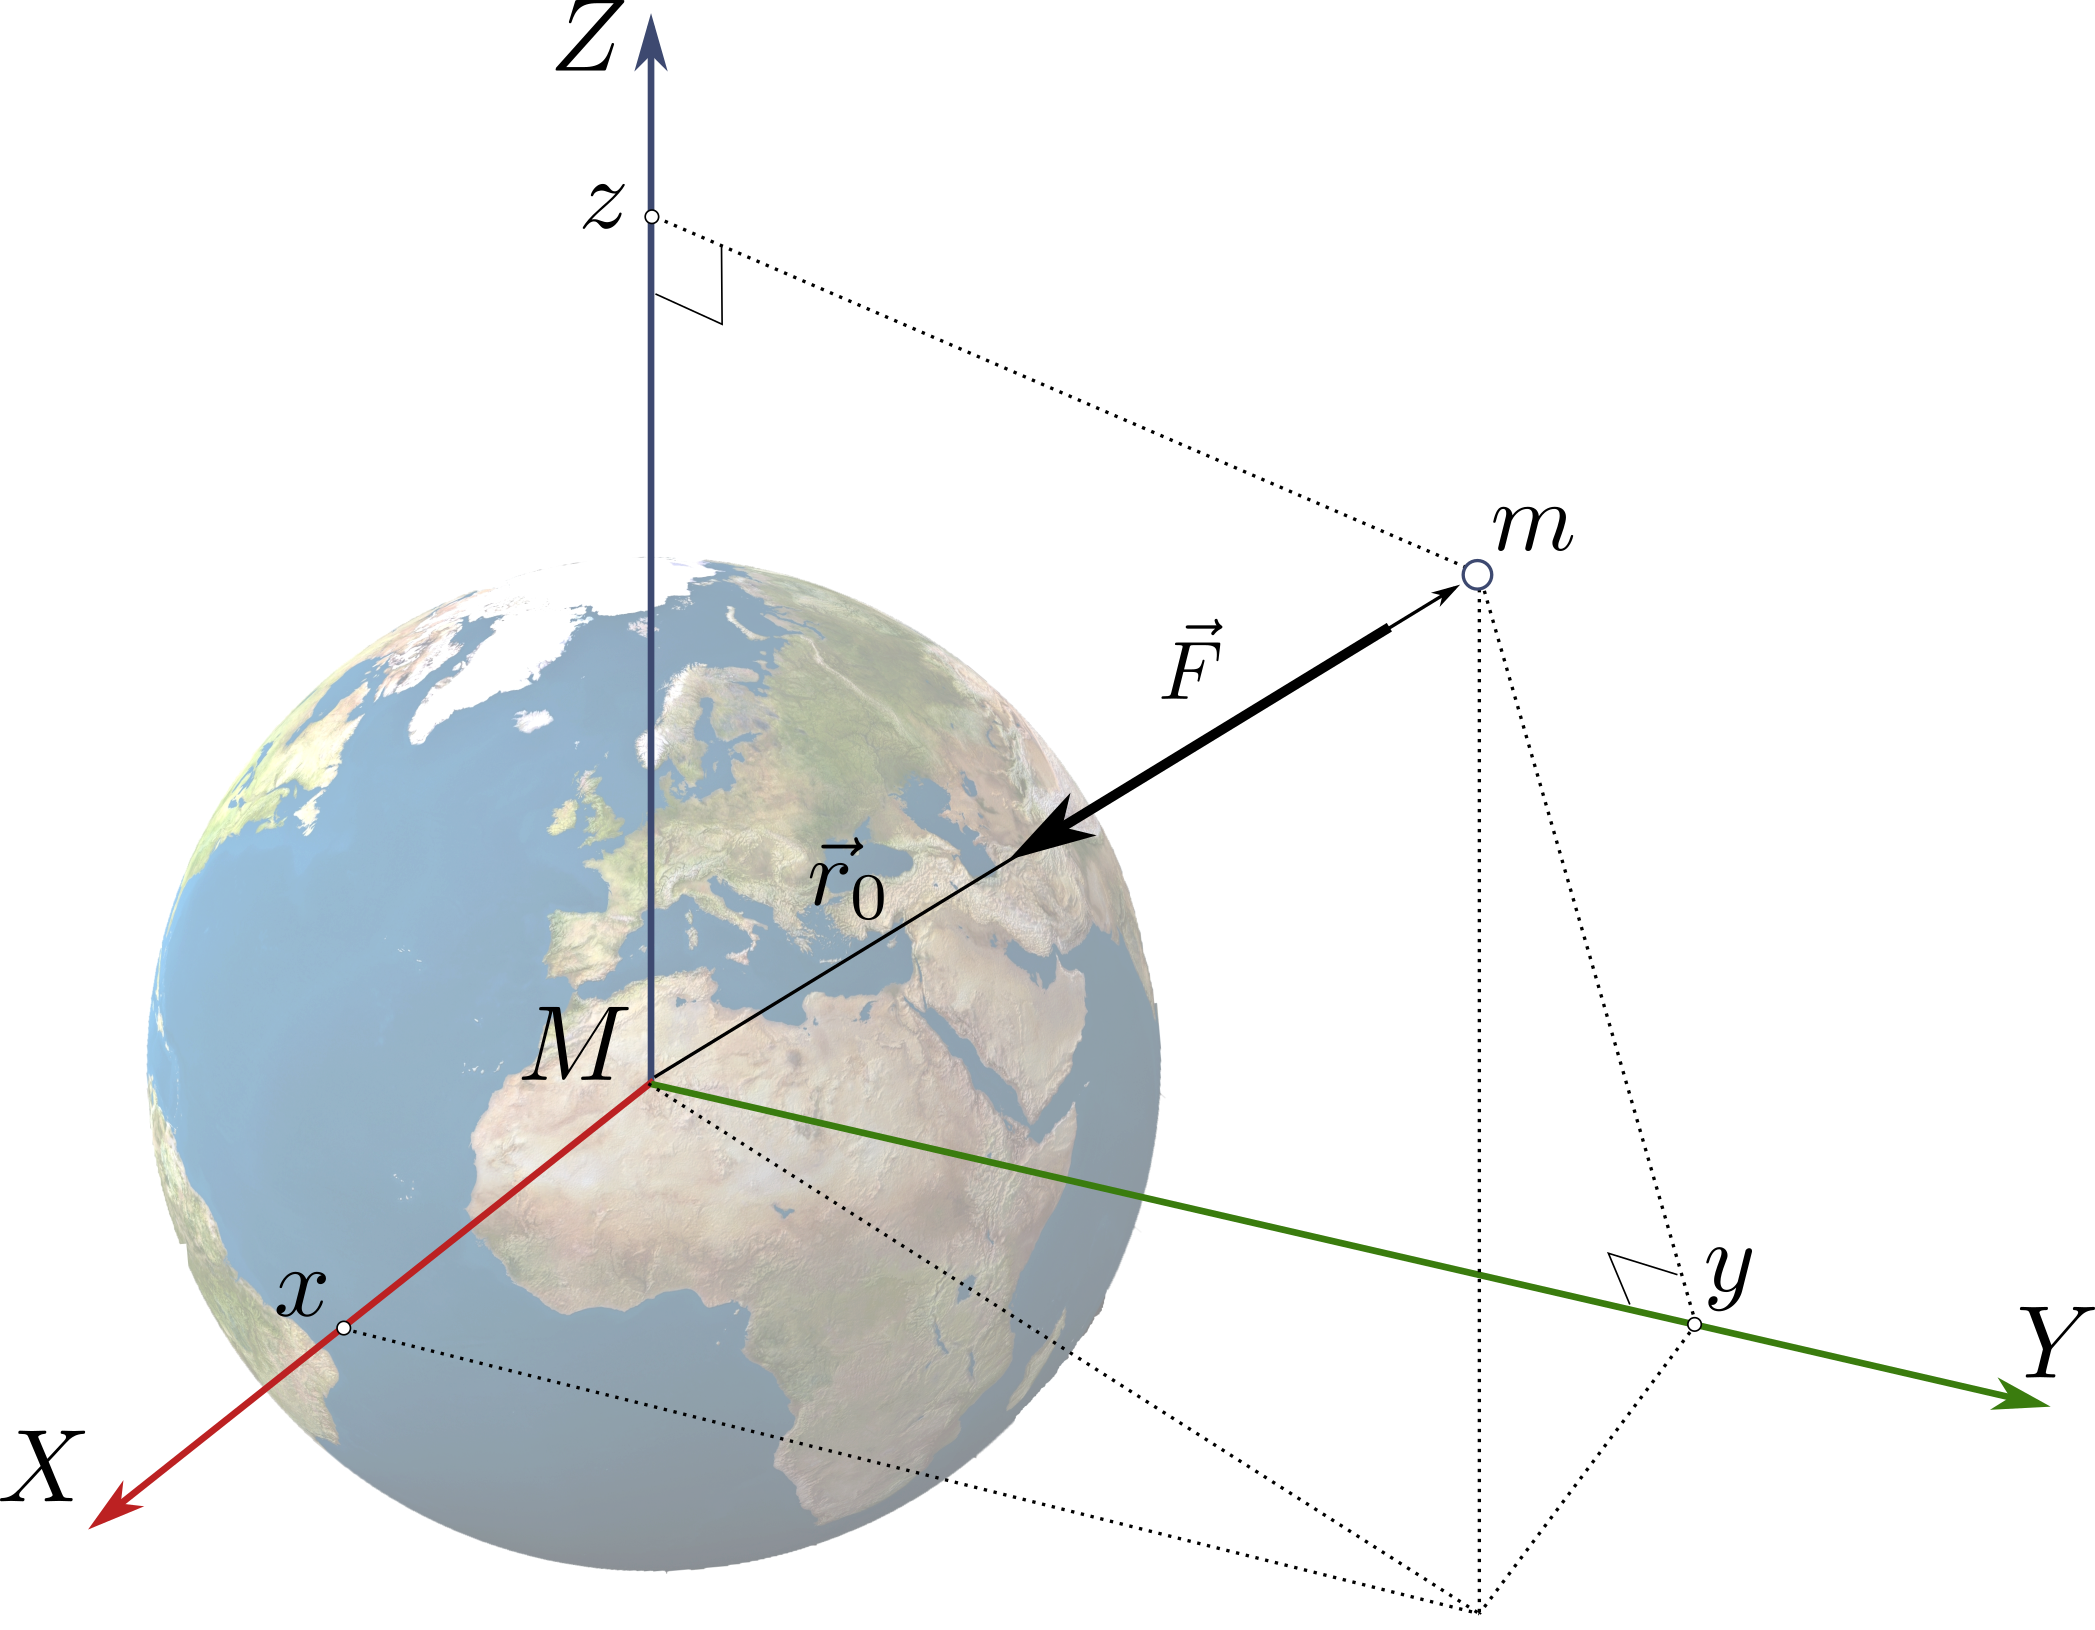
\includegraphics[width=0.8\textwidth]{ECI.png}  
\end{figure}
\end{frame}


\begin{frame}[fragile]{Векторное уравнение движения}
$$
  m \vec a = \vec F
$$
Модуль силы притяжения Земли, действующей на спутник:
$$
  |\vec F| = F = G \frac{M m}{r_0^2} = \mu \frac{m}{r_0^2}, 
$$ 
где
$$ 
\mu = G M \approx 3.986\cdot 10^{14} \text{ м}^3/\text{c}^2
$$ 
гравитационный параметр Земли
\end{frame}


\begin{frame}[fragile]{Координатная запись}
$$
\begin{aligned}
  & m a_x = F_x = - F \cos (\widehat{X,-\vec F}) = - F \cos (\widehat{X, r_0}) = - F \cdot{\;} \frac{x}{r_0}, \\
  & m a_y = F_y = - F \cos (\widehat{Y,-\vec F}) = - F \cos (\widehat{Y, r_0}) = - F \cdot \frac{y}{r_0}, \\
  & m a_z = F_z = - F \cos (\widehat{Z,-\vec F}) = - F \cos (\widehat{Z, r_0}) = - F \cdot \frac{z}{r_0}.
\end{aligned}
$$
\end{frame}

\begin{frame}[fragile]{Уравнения движения}
$$
\begin{aligned}
  & \boxed{m a_x} = m \frac{d^2 x}{dt^2} = F_x = - F \cdot \frac{x}{r_0} = - \mu \frac{m}{r_0^2} \; \frac{x}{r_0} = \boxed{- \mu \frac{m \cdot x}{r_0^3}}, \\
  & \\
  & \boxed{m a_y} = m \frac{d^2 y}{dt^2} = F_y = - F \cdot \frac{y}{r_0} = - \mu \frac{m}{r_0^2} \; \frac{y}{r_0} = \boxed{- \mu \frac{m \cdot y}{r_0^3}}, \\
  & \\
  & \boxed{m a_z} = m \frac{d^2 z}{dt^2} = F_z = - F \cdot \frac{z}{r_0} = - \mu \frac{m}{r_0^2} \; \frac{z}{r_0} = \boxed{- \mu \frac{m \cdot z}{r_0^3}}.
\end{aligned}
$$
$$
r_0 = \sqrt{x^2 + y^2 + z^2}
$$
\end{frame}

%\begin{frame}[fragile]{Элементы орбиты}
%\begin{columns}
%\column{0.6\linewidth}
%\begin{figure}[htbp]
%  \centering
%  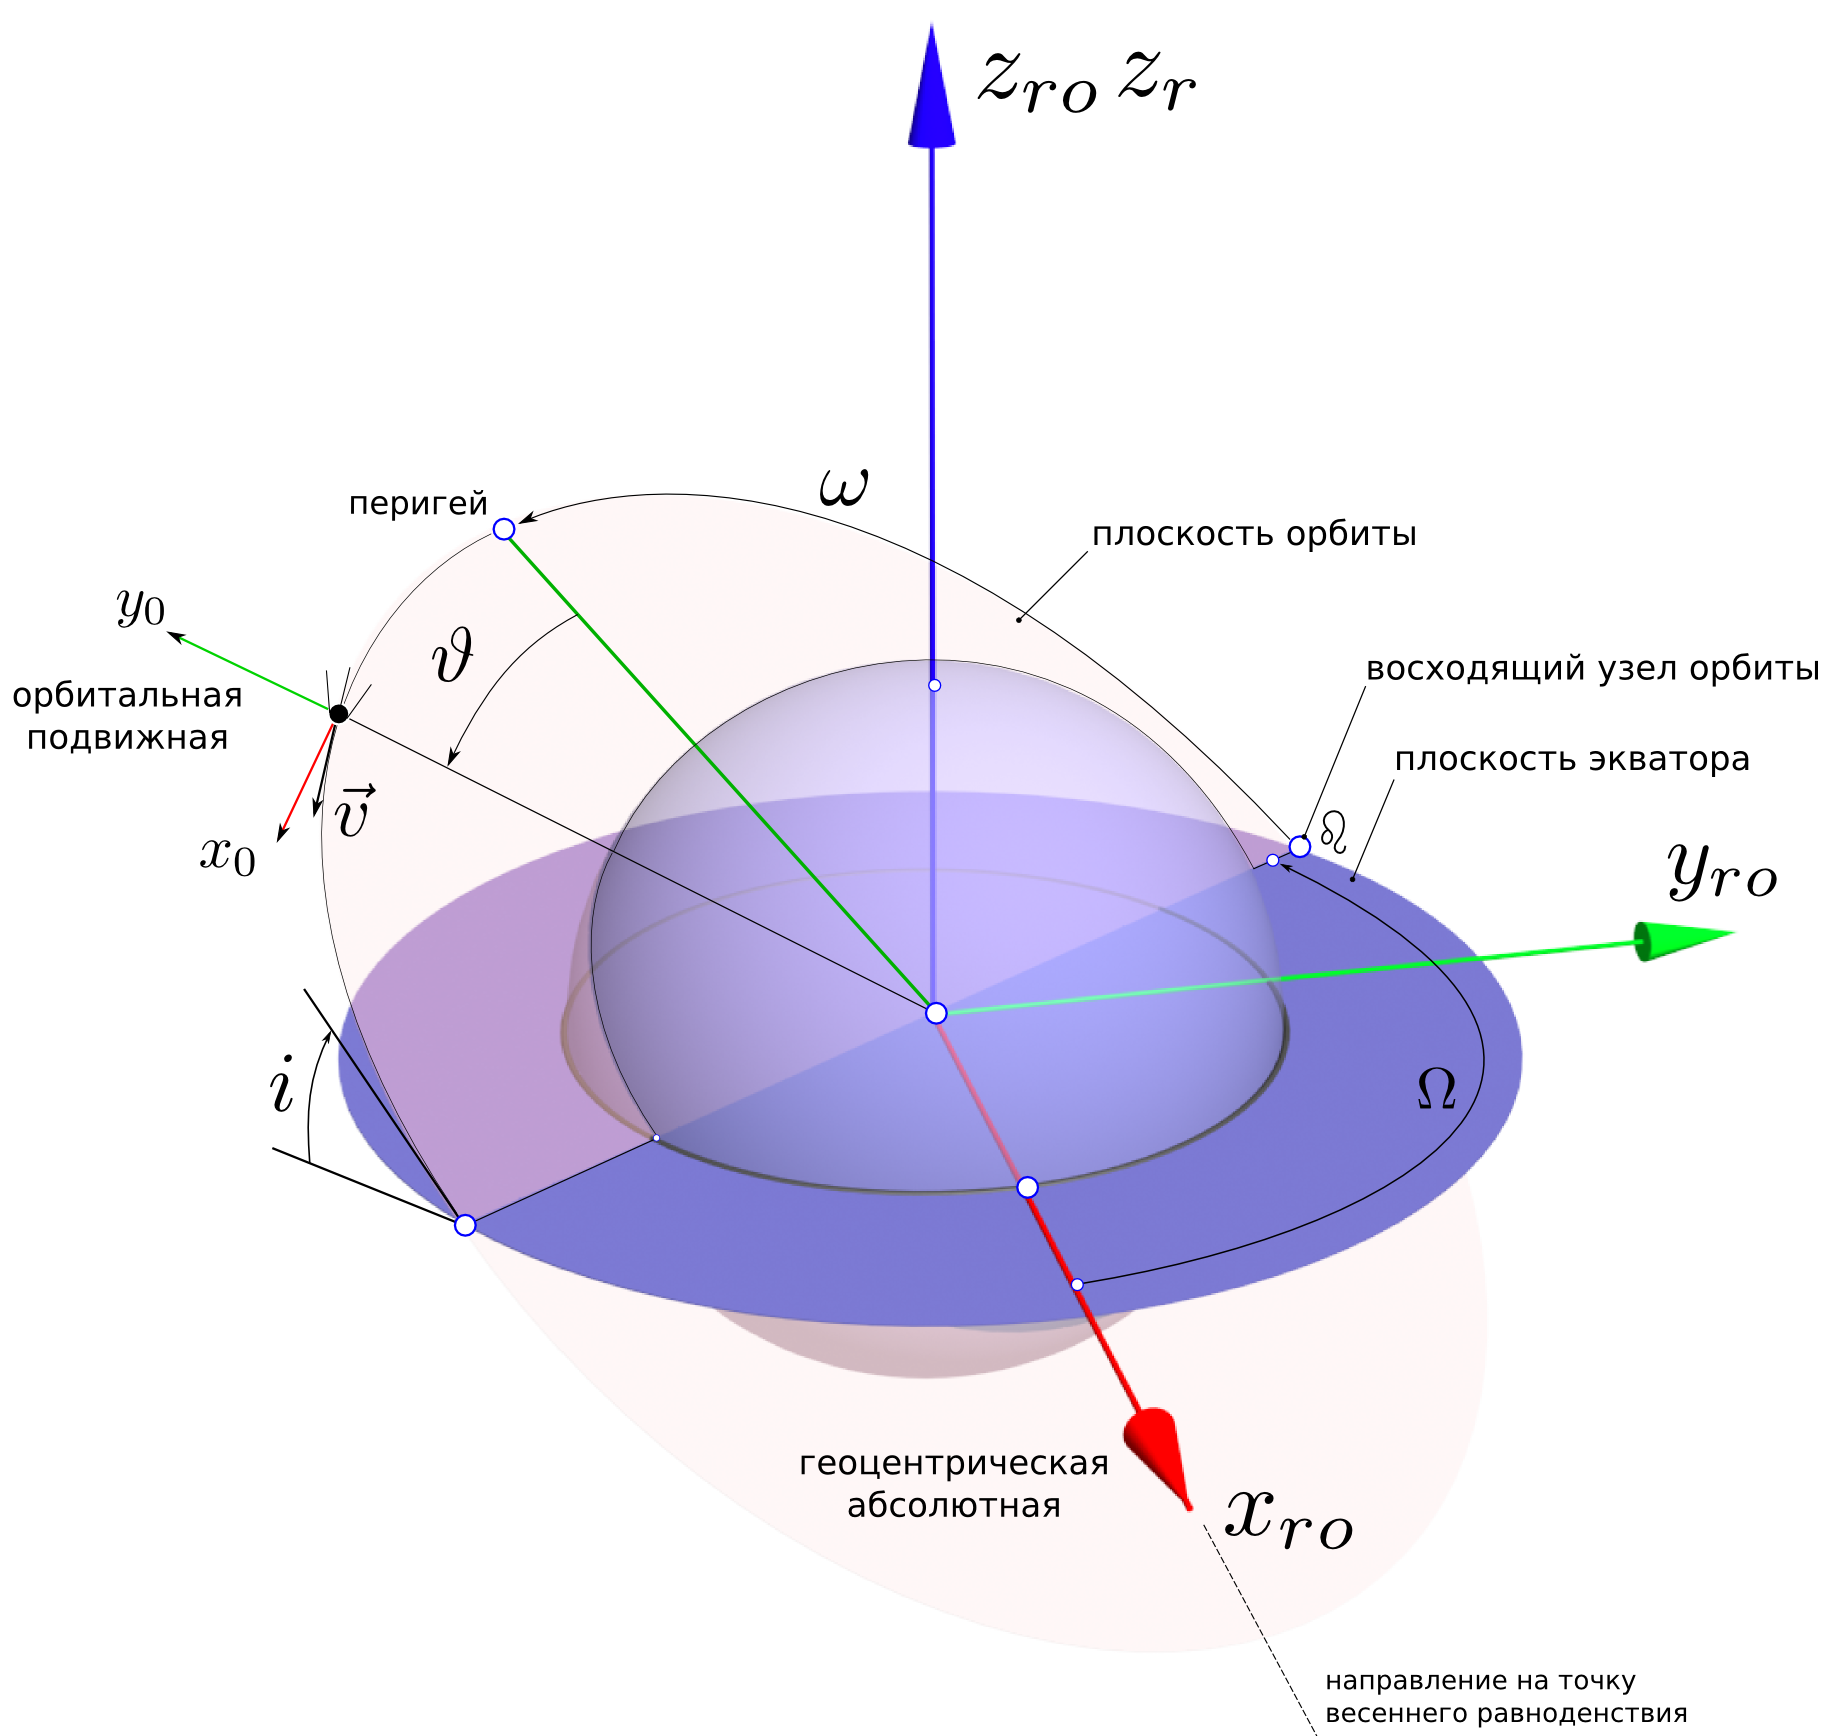
\includegraphics[width=1\textwidth]{orbit.png}
%\end{figure}
%\column{0.4\linewidth}
%\begin{itemize}
%  \item $a$ -- большая полуось,
%  \item $i$ -- наклонение,
%  \item $e$ -- эксцентриситет,
%  \item $\Omega$ -- долгота восходящего узла,
%  \item $\omega$ -- аргумент перицентра,
%  \item $\vartheta$ -- угол истинной аномалии,  
%\end{itemize}
%\end{columns}
%\end{frame}

\begin{frame}[fragile]{Приведение к ОДУ первого порядка}
$$
\left\{
\begin{aligned}
  & m a_x = F_x, \\
  & m a_y = F_y, \\
  & m a_z = F_z.
\end{aligned}\right. \quad \Rightarrow \quad
\left\{
\begin{aligned}
  & \dot v_x = F_x/m = - \mu \, x / r_0^3, \\
  & \dot v_y = F_y/m = - \mu \, y / r_0^3, \\
  & \dot v_z = F_z/m = - \mu \, z / r_0^3, \\
  & \dot x = v_x, \\
  & \dot y = v_y, \\
  & \dot z = v_z 
\end{aligned}
\right.
$$
Неизвестные функции: 
$$
  v_x, v_y, v_z, x, y, z
$$
\end{frame}

\begin{frame}[fragile]{Файл-функция правой части dqdt.m}
Вектор состояния:
$$
  q = (v_x, v_y, v_z, x, y, z)
$$
\begin{lstlisting}
function dq = dqdt(t, q) 
  global params;
  v = q(1:3);
  r = q(4:6);  
  % Вектор ускорения
  a = - params.mu*r/norm(r,2)^3;
  % Возвращаем производную вектора q
  dq = [a,v];
\end{lstlisting}
\end{frame}

\begin{frame}[fragile]{Главный файл-скрипт orbitalMotion.m}
\begin{lstlisting}
% |\lstcomment{Гравитационный параметр Земли}|
params.mu=3.986e14;
% |\lstcomment{Радиус Земли}|
params.Rz = 6371000;    
% |\lstcomment{Формируем вектор начальных условий}|
% |\lstcomment{для круговой орбиты высотой}|
h  = 300000;
% |\lstcomment{Орбитальная скорость}|
V  = sqrt(params.mu/(params.Rz+h));  
q0 = [0;V;0;h+Rz;0;0];
% |\lstcomment{От 0 до одного орбитального периода}|
tk = 2*pi*(h+params.Rz)/V;
% |\lstcomment{Вызываем функцию интегрирования}|
[t,q] = ode45(@dqdt, q0, [0 tk]);  
\end{lstlisting}
\end{frame}



\begin{frame}[fragile]{Файл-функция правой части dqdt.m}
Вариант функции правых частей с передачей параметров
\begin{lstlisting}
function dq = dqdt(t, q, params)   
  v = q(1:3);
  r = q(4:6);  
  % Вектор ускорения
  a = - params.mu*r/norm(r,2)^3;
  % Возвращаем производную вектора q
  dq = [a,v];
\end{lstlisting}
\end{frame}

\begin{frame}[fragile]{Главный файл-скрипт orbitalMotion.m}
\begin{lstlisting}
% |\lstcomment{Гравитационный параметр Земли}|
params.mu=3.986e14;
% |\lstcomment{Радиус Земли}|
params.Rz = 6371000;    
% |\lstcomment{Формируем вектор начальных условий}|
% |\lstcomment{для круговой орбиты высотой}|
h  = 300000;
% |\lstcomment{Орбитальная скорость}|
V  = sqrt(params.mu/(params.Rz+h));  
q0 = [0;V;0;h+Rz;0;0];
% |\lstcomment{От 0 до одного орбитального периода}|
tk = 2*pi*(h+params.Rz)/V;
% |\lstcomment{Вызываем функцию интегрирования}|
[t,q] = ode45(@(t,q) dqdt(t,q,params),q0,[0 tk]);  
\end{lstlisting}
\end{frame}






\begin{frame}[fragile]{Результат интегрирования}
После выполнения строки
\begin{lstlisting}
[t,q] = ode45(@dqdt, q0, [0 tk]);  
\end{lstlisting}
Матрица $q$ будет содержать 6 столбцов и число строк, равное числу шагов интегрирования, соответсвующие моментам времени, содержащимися в столбце $t$:
$$
  t = \begin{bmatrix} 0 \\ t_1 \\ t_2 \\ \ldots \\ t_n \end{bmatrix}, \quad
  q = 
\begin{bmatrix} 
  v_{x0} & v_{y0} & v_{z0} & x_{0} & y_{0} & z_{0} \\
  v_{x1} & v_{y1} & v_{z1} & x_{1} & y_{1} & z_{1} \\
  v_{x2} & v_{y2} & v_{z2} & x_{2} & y_{2} & z_{2} \\
  \ldots & \ldots & \ldots & \ldots & \ldots & \ldots \\
  v_{xn} & v_{yn} & v_{zn} & x_{n} & y_{n} & z_{n} 
\end{bmatrix}.
$$
\end{frame}

\begin{frame}[fragile]{Экспорт результатов в текстовый файл}
Для обработки результатов в других программах возможна запись таблицы с результатами в текстовый файл, в котором значения в каждой строке разделяются запятой:
\begin{lstlisting}  
  dlmwrite('results.csv',[t, q], ',');
\end{lstlisting}
$$
\begin{bmatrix} 
  t_0, & v_{x0}, & v_{y0}, & v_{z0}, & x_{0}, & y_{0}, & z_{0}, \\
  t_1, & v_{x1}, & v_{y1}, & v_{z1}, & x_{1}, & y_{1}, & z_{1}, \\
  t_2, & v_{x2}, & v_{y2}, & v_{z2}, & x_{2}, & y_{2}, & z_{2}, \\
  \ldots & \ldots & \ldots & \ldots & \ldots & \ldots & \ldots \\
  t_n, & v_{xn}, & v_{yn}, & v_{zn}, & x_{n}, & y_{n}, & z_{n} 
\end{bmatrix}.
$$
\end{frame}


\begin{frame}[fragile]{Построение графиков}
\matcode{Файл orbitalMotion.m}
\begin{lstlisting}
  plot(t, (sqrt(sum(q(4:6,:).^2,2))-Rz)*0.001);
  xlabel('t, c');
  ylabel('r, км');
\end{lstlisting}

\end{frame}


%
%
%
\section{Пересчёт координат из геоцентрической СК в орбитальную подвижную}
%
%
%
\begin{frame}[fragile]{Направления осей $Cx_oy_oz_o$}
\begin{columns} 
\column{0.5\linewidth} 
\begin{center}
 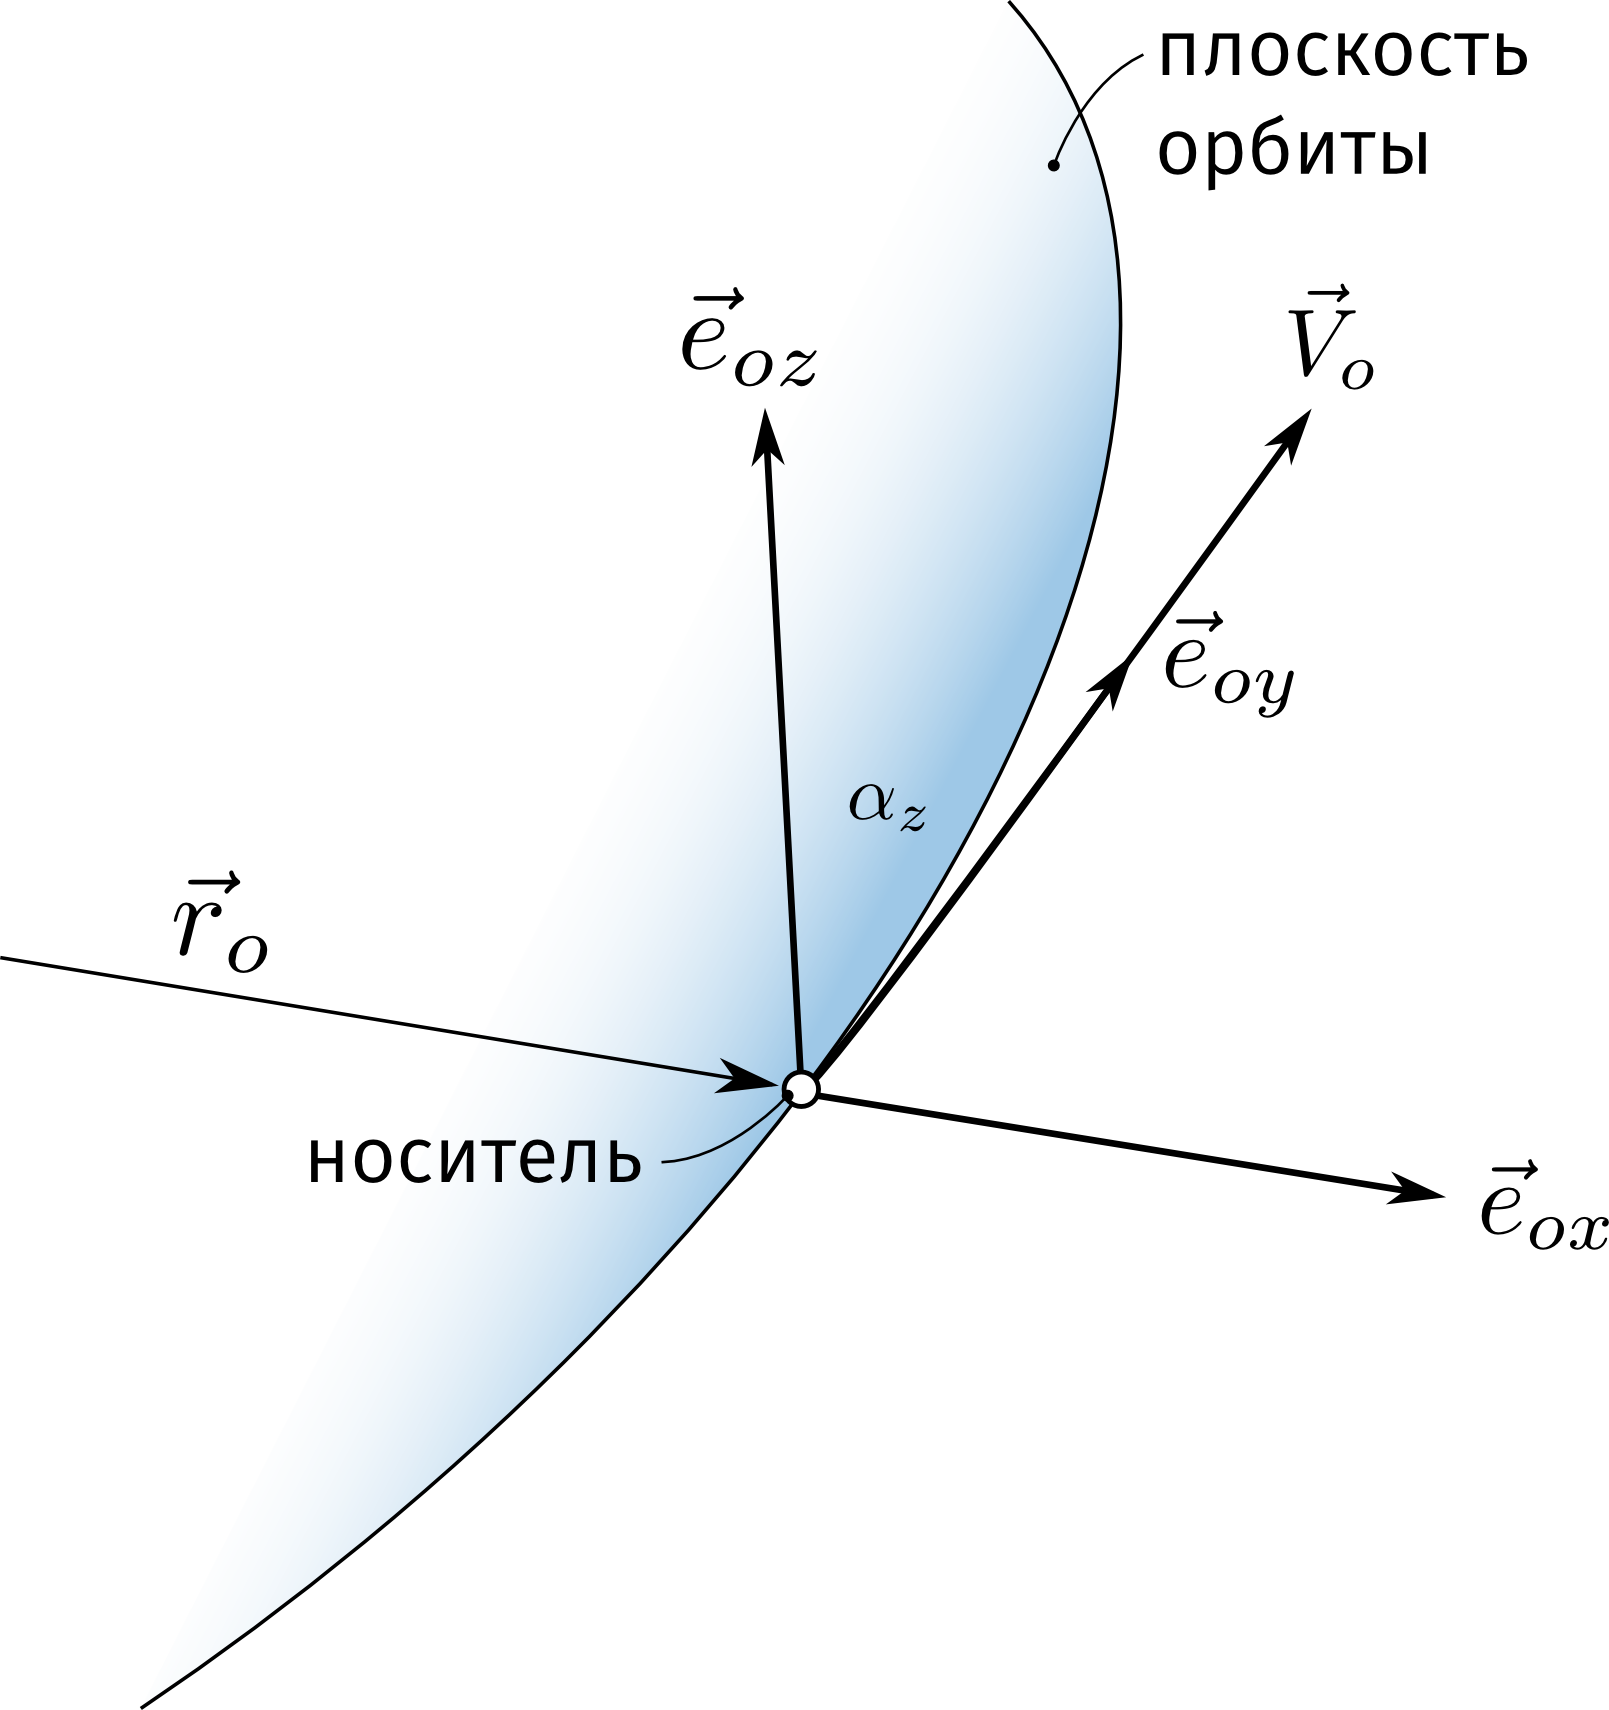
\includegraphics[width=1.0\linewidth]{./orbitalCoordinatesOnly.png} 
\end{center}
\column{0.5\linewidth} 
Единичный вектор радиус-вектора носителя:
$$
\vec e_{ox} = \vec r_0 / r_0.
$$
Единичный вектор нормали к орбите:
$$
\vec e_{oz} = (\vec r_0 \times \vec v_0) / | \vec r_0 \times \vec v_0 |.
$$
Единичный вектор трансверсали:
$$
\vec e_{oy} = (\vec e_{oz} \times \vec e_{ox})/| \vec e_{oz} \times \vec e_{ox} |.
$$
\end{columns}
\end{frame}


\begin{frame}[fragile]{Положение КА относительно носителя}
\begin{columns} 
\column{0.5\linewidth} 
\begin{center}
 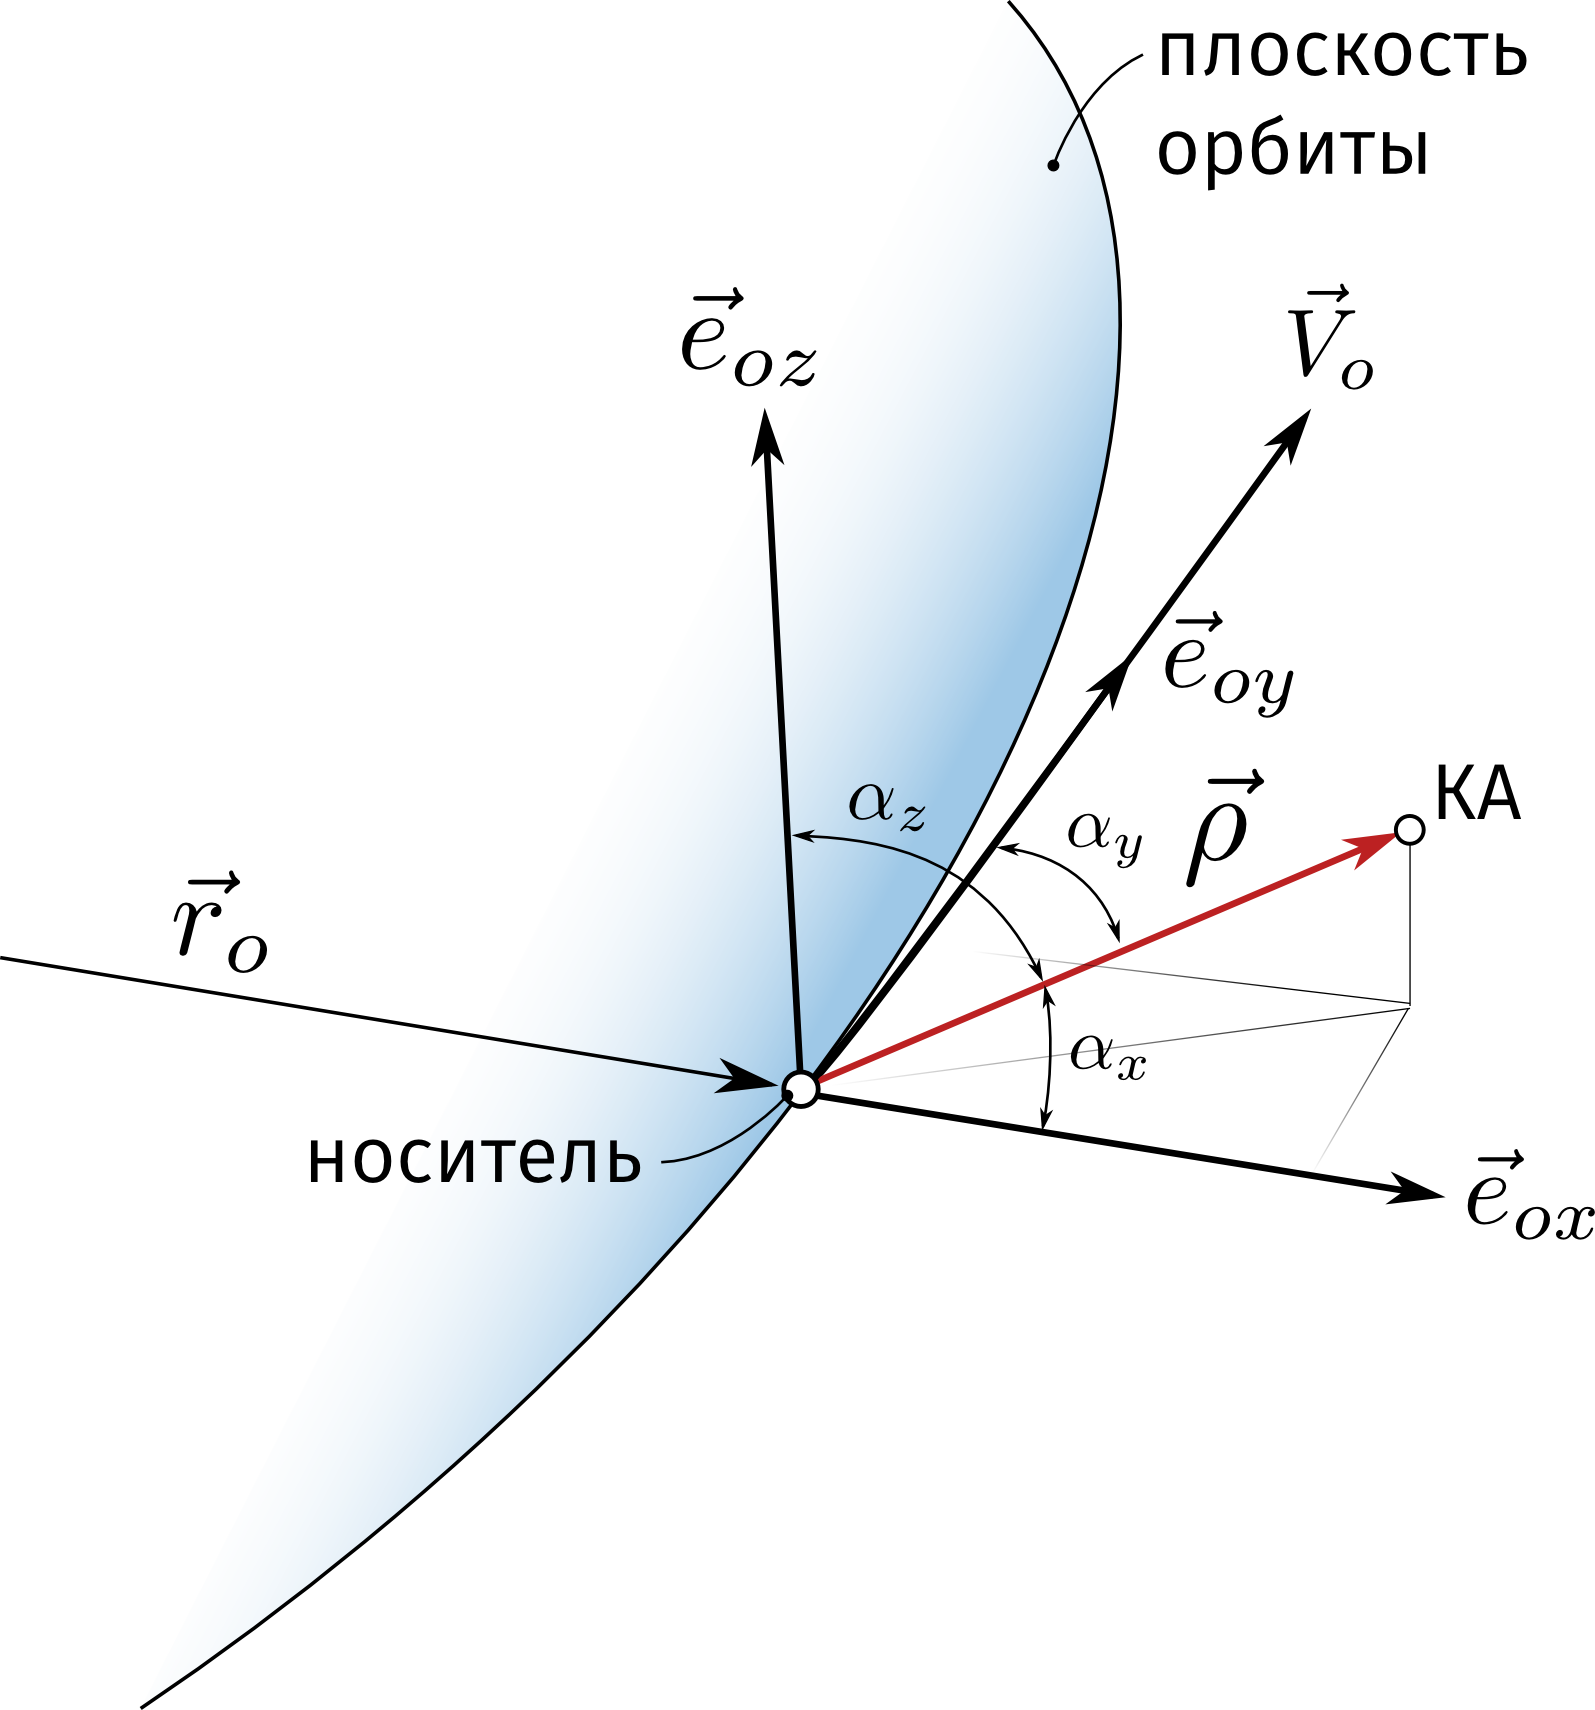
\includegraphics[width=1.0\linewidth]{./orbitalCoordinates.png} 
\end{center}
\column{0.5\linewidth} 
Радиус-вектор положения КА относительно носителя:
$$
\vec \rho = \vec r - \vec r_0
$$
Координаты КА относительно носителя в $Cx_oy_oz_o$:
$$
\begin{aligned}
  & x = \vec \rho \cdot \vec e_{ox}=\vec \rho \cos \alpha_x, \\
  & y = \vec \rho \cdot \vec e_{oy}=\vec \rho \cos \alpha_y, \\
  & z = \vec \rho \cdot \vec e_{oz}=\vec \rho \cos \alpha_z.
\end{aligned}
$$
\end{columns}
\end{frame}


\begin{frame}[fragile]{Вектор относительного положения}
Матрица результатов интегрирования абсолютного движения двух материальных точек:
\begin{lstlisting}
q = 
v1x, v1y, v1z, x1, y1, z1, v2x, v2y, v2z, x2, y2, z2
v1x, v1y, v1z, x1, y1, z1, v2x, v2y, v2z, x2, y2, z2
...
\end{lstlisting}
Координатный столбец вектора положения второй точки относительно первой в проекциях на неподвижную систему координат:
\begin{lstlisting}
rho = q(:,10:12)-q(:,1:3);
\end{lstlisting}
\end{frame}

\begin{frame}[fragile]{Орты орбитальной подвижной системы}
\begin{lstlisting}
q = 
v1x, v1y, v1z, x1, y1, z1, v2x, v2y, v2z, x2, y2, z2
v1x, v1y, v1z, x1, y1, z1, v2x, v2y, v2z, x2, y2, z2
...
\end{lstlisting}
Координатные столбцы единичных векторов орбитальной подвижной системы координат, связанной с первым телом:
\begin{lstlisting}
r = sqrt( sum( q(:,4:6).*q(:,4:6) ,2) );
ex0 = q(:,4:6)./repmat(r,1,3);
\end{lstlisting}
\begin{lstlisting}[firstnumber=last]
v = sqrt( sum( q(:,1:3).*q(:,1:3) ,2) );
ev0 = q(:,4:6)./repmat(v,1,3);
\end{lstlisting}
\end{frame}

\begin{frame}[fragile]{Орты орбитальной подвижной системы}
\begin{lstlisting}
q = 
v1x, v1y, v1z, x1, y1, z1, v2x, v2y, v2z, x2, y2, z2
v1x, v1y, v1z, x1, y1, z1, v2x, v2y, v2z, x2, y2, z2
...
\end{lstlisting}
Единичный вектор нормали к плоскости орбиты:
\begin{lstlisting}
ez0 = cross(ex0,ev0,2);
ez0 = ez0./repmat(sqrt(sum(ez0.*ez0,2)),1,3);
\end{lstlisting}
Единичный вектор трансверсали:
\begin{lstlisting}[firstnumber=last]
ey0 = cross(ez0,er0,2);
ey0 = ey0./repmat(sqrt(sum(ey0.*ey0,2)),1,3);
\end{lstlisting}
\end{frame}



\begin{frame}[fragile]{Относительное положение}
Координатный столбец вектора положения второй точки относительно первой в проекциях на неподвижную систему координат:
\begin{lstlisting}
rho = q(:,10:12)-q(:,1:3);
\end{lstlisting}
Тот же вектор в проекция на оси орбитальной подвижной системы:
\begin{lstlisting}
rho_o = [dot(rho,ex0,2),dot(rho,ey0,2),dot(rho,ez0,2)];
\end{lstlisting}
\end{frame}



\begin{frame}{Задание}
\begin{itemize}
  \item Используя программу численного интегрирования движения спутника в центральном поле определить движение спутника-носителя относительно геоцентрической инерциальной системы координат с начальными условиями, соответствующими его движению по круговой орбите высотой 800 км.
\end{itemize}
\end{frame}

\begin{frame}{Задание}
\begin{itemize}
  \item Второй спутник отделяется от первого со скоростью 1 м/с в направлении вектора орбитальной скорости. Определить движение второго спутника относительно геоцентрической инерциальной системы координат.
  \item Построить траекторию движения второго спутника \emph{относительно} первого в орбитальной подвиженой системе коордиант $Ox_oy_oz_o$. Начало орбитальной подвижной системы координат расположеное в центре масс первого спутника (точка O). 
\end{itemize}
\end{frame}

\begin{frame}{Орбитальная подвижная СК}
\begin{itemize}
  \item Ось $Ox_o$ направлена из вдоль радиус-вектора первого спутника относительно центра Земли (``вверх''). 
  \item Ось $Oy_o$ лежит в плоскости орбиты и направлена в сторону орбительной скорости первого спутника. 
  \item Ось $Oz_o$ дополняет систему до правой.
\end{itemize}  
\end{frame}

\begin{frame}{Орбитальная подвижная СК}
\begin{figure}[htbp]
  \centering
  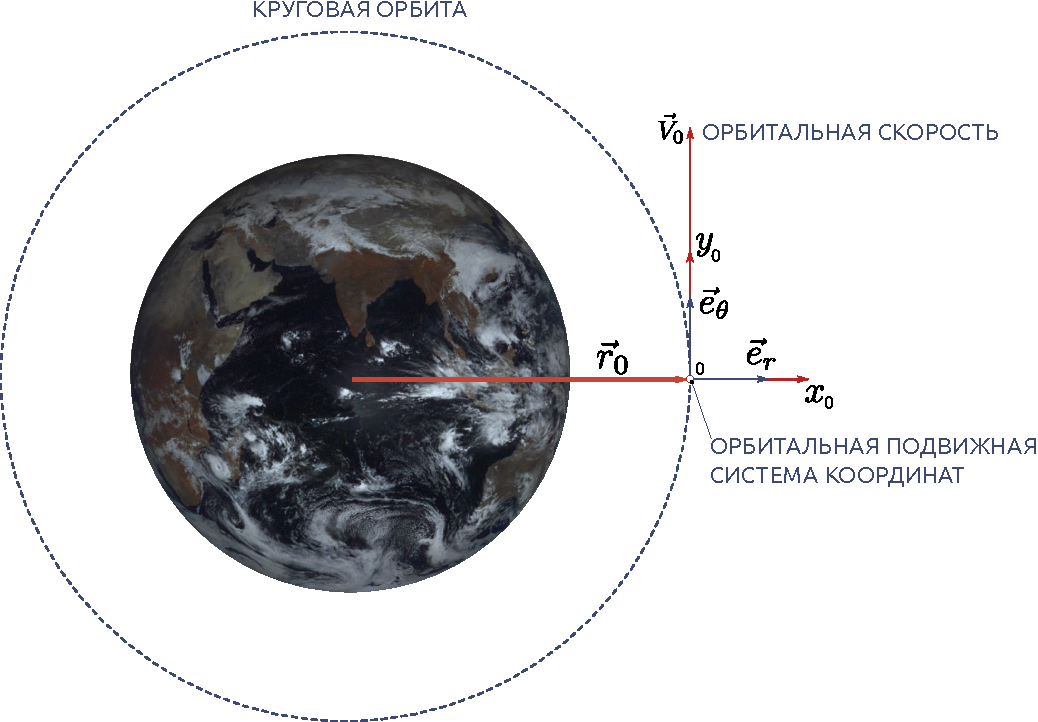
\includegraphics[width=0.95\textwidth]{Orbital_SC.pdf}
\end{figure}
\end{frame}

 
\end{document}
